% This must be in the first 5 lines to tell arXiv to use pdfLaTeX, which is strongly recommended.
\pdfoutput=1
% In particular, the hyperref package requires pdfLaTeX in order to break URLs across lines.

\documentclass[11pt]{article}
\usepackage{graphicx}
\usepackage{wrapfig}

% Remove the "review" option to generate the final version.
\usepackage[]{ACL2023}

% Standard package includes
\usepackage{times}
\usepackage{latexsym}

% For proper rendering and hyphenation of words containing Latin characters (including in bib files)
\usepackage[T1]{fontenc}
% For Vietnamese characters
% \usepackage[T5]{fontenc}
% See https://www.latex-project.org/help/documentation/encguide.pdf for other character sets

% This assumes your files are encoded as UTF8
\usepackage[utf8]{inputenc}

% This is not strictly necessary, and may be commented out.
% However, it will improve the layout of the manuscript,
% and will typically save some space.
\usepackage{microtype}

% This is also not strictly necessary, and may be commented out.
% However, it will improve the aesthetics of text in
% the typewriter font.
\usepackage{inconsolata}


% If the title and author information does not fit in the area allocated, uncomment the following
%
%\setlength\titlebox{<dim>}
%
% and set <dim> to something 5cm or larger.

\title{Assessing the Impact Score of Scientific Publications through the Analysis of Abstracts and their Metadata}


\author{Artem Lebedev\\
  UC Berkeley / Berkeley, CA \\
  \texttt{artem.lebedev@berkeley.edu} \\\And
 Farouk Ghandour \\
  UC Berkeley / Berkeley, CA \\
  \texttt{fghandour18@berkeley.edu} \\}

\begin{document}
\maketitle
\begin{abstract}
An impact score of the academic paper is a metric critically important for a scientist's career and attraction of funding for future research. The ability to predict the potential score of a paper could help scientists adjust their presentation strategy to achieve maximum impact. Natural language processing (NLP) is a logical tool to examine what leads to a scientific article's strong impact score because it allows one to analyze an article’s content numerically. In this paper we demonstarte the use of sciBERT with a combination of convolutional neural net to predict the impact factor of the paper based on it abstract.
\end{abstract}

\section{Introduction}
% Not done. Supppoesed to describe motivation for the work.
An impact score of the academic paper is a metric critically important for a scientist's career and attraction of funding for future research. The ability to predict the potential score of a paper could help scientists adjust their presentation strategy to achieve maximum impact. Our team aims to elucidate the factors that drive acceptance in high-impact journals. The main challenge of this task is that acceptance of a paper is a product of the interplay between the features of the paper and the journal. Statistically speaking, interaction terms in the model have relatively large weights and some interaction terms are likely non-linear. 
% Not done

\section{Background}
% Not done. Supppoesed to describe motivation for the work.
This is where we discuss background literature. \citep{hs2022}
% Not done

\section{Data}
% Not done. Supppoesed to describe motivation for the work.
Brief description of data
\subsection{ETL}
Short description of how downloaded data was transformed into final dataframe. 
\subsection{EDA}
Appendix~\ref{sec:appendix} will contain full EDA

\begin{figure}
	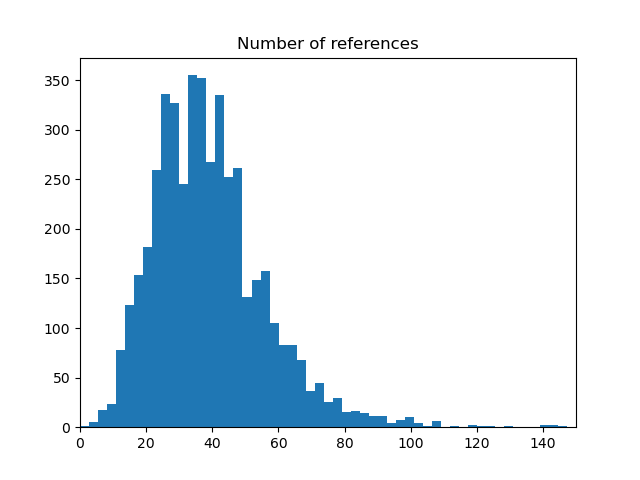
\includegraphics[width= \columnwidth]{./Images/Ref_hist.png}
	\caption{Distribution of the number of cited references}
	\label{fig:img1}
\end{figure}
% Not done

\begin{table}
\centering
\begin{tabular}{lc}
\hline
\textbf{Command} & \textbf{Output}\\
\hline
\verb|{\`i}| & {\`i} \\ 
\verb|{\.I}| & {\.I} \\ 
\verb|{\o}| & {\o} \\
\verb|{\aa}| & {\aa}  \\\hline
\end{tabular}
\begin{tabular}{lc}
\hline
\textbf{Command} & \textbf{Output}\\
\hline 
\verb|{\l}| & {\l} \\ 
\verb|{\~n}| & {\~n} \\ 
\verb|{\H o}| & {\H o} \\ 
\verb|{\v r}| & {\v r} \\ 
\hline
\end{tabular}
\caption{Example commands for accented characters, to be used in, \emph{e.g.}, Bib\TeX{} entries.}
\label{tab:accents}
\end{table}


\section*{Limitations}
While we are open to different types of limitations, just mentioning that a set of results have been shown for English only probably does not reflect what we expect. 
Mentioning that the method works mostly for languages with limited morphology, like English, is a much better alternative.
In addition, limitations such as low scalability to long text, the requirement of large GPU resources, or other things that inspire crucial further investigation are welcome.

% Entries for the entire Anthology, followed by custom entries
\bibliography{custom}
\bibliographystyle{acl_natbib}

\appendix

\section{Example Appendix}
\label{sec:appendix}

This is a section in the appendix.

\end{document}
